\section{An overview on Universality}

It is well know among physicists and mathematicians alike that random independent phenomena share a common characteristics when we are dealing with large quantities. This is formally expressed in terms of the central limit theorem: Take $\{x_n\}_{n\geq1}$ i.i.d, then, if we center and scale the variables $x_n \rightarrow y_n \deff (x_n - \E(x_n)) / \sqrt{\Var(x_n)}$, then we have the limit
\begin{equation}
	\lim_{n\rightarrow \infty} \p\left( \frac{\sum_{k=1}^{n} y_k}{\sqrt{n}} \leq t \right) = \int_{-\infty}^t \ee^{-\frac{u^2}{2}} \frac{\dd u}{\sqrt{2\pi}}.
\end{equation} 
This in an amazing result as it appoints the Gaussian distribution as a universal distribution for great numbers of uncorrelated random processes.  There is however, many phenomena where these assumptions can't hold. This is very natural for the many interacting physical systems or mathematical models such as roots of polynomials, where the points 'show repulsion'. For these cases another Universality result must be considered, one where the Gaussian distribution is substituted with a more appropriate distribution: The Tracy-Widow,
\begin{equation}
	\lim_{n\rightarrow \infty} \p\left( \frac{\sum_{k=1}^{n} \left( \lambda_k - z_n^{(\beta)}\right)}{s^{(\beta)}_n} \leq t \right) = \F_{\beta}(t)
\end{equation}
where $s_n^{(\beta)}$ has something to do with the class of the problem - gives the scale needed, and $F_\beta(t)$ is the cumulative distribution given by the ($\beta$)-Tracy-Widow

\subsection{Modeling by Random Matrices}

An amazing source for a brief introduction - and the main source used for a number of the examples if the great overview in \cite{deift2006universalitymathematicalphysicalsystems}, by Deift in $2006$. For the meaning of what is going to be the main subset of this chapter - modeling by a Random Matrix Model - we cite an analogy given by this same work.
\\

\begin{sic}
	(Deif)
	This procedure can  be viewed as follows: A scientist wishes to investigate some statistical phenomenon. What s’he has at hand is a microscope and a handbook of matrix ensembles. The data $\{a_k\}$ are embedded on a slide which can be inserted into the microscope. The only freedom that the scientist has is to center the slide, $a_k \rightarrow a_k - A$, and then adjust the focus $a_k - A \rightarrow \tilde{a}_k = \gamma_a(a_k - A)$ so that on average one data point $\tilde{a}_k$ appears per unit length on the slide. At that point the scientist takes out his’r handbook, and then tries to match the statistics of the $\tilde{a}_k$’s with those of the eigenvalues of some ensemble. If the fit is good, the scientist then says that the system is well-modeled by RMT.
\end{sic}

\section{Heavy Atom Nuclei}

This seciton is based on \cite{deift2006universalitymathematicalphysicalsystems}. 

Consider the scattering of neutrons of a heavy nucleus, say uranium $U^{238}$. The scattering cross-section is plotted as a function of the energy $E$ of the incoming neutrons, and one obtains a jagged graph with many hundreds of sharp peaks $E-1 < E_2 < \cdots$  and valleys $E'_1 < E'_2 < \cdots $. If $E \approx E_j$ for some $j$, the neutron is strongly repelled from the nucleus, and if $E \approx E'_j$ for some $j$, then the neutron sails through the nucleus, essentially unimpeded. The $E_j$’s are called scattering resonances. The challenge faced by physicists in the late $40$’s and early $50$’s was to develop an effective model to describe these resonances. One could of course write down a Schrodinger-type equation for the scattering system, but because of the high dimensionality of the problem there is clearly no hope of solving the equation for the $E_j$’s either analytically or numerically. However, as more experiments were done on heavy nuclei, each with hundreds of $E_j$’s, a consensus began to emerge that the “correct” theory of resonances was statistical, and here Wigner led the way. Any efefctive theory would have to incorporate two essential features present in the data, i.e.
\begin{enumerate}
 \item Modulo certain natural symmetry considerations, all nuclei in the same symmetry class exhibited universal behavior;
 \item In all cases, the $E_j$’s exhibited repulsion, or, more precisely, the probability that two $E_j$’s would be close together was small. 
\end{enumerate}

\begin{sic}
	(Eugene Wigner - On the Wigner Surmise (1956))
	“Perhaps I am now too courageous when I try to guess the distribution of the distances between successive levels (of energies of heavy nuclei). Theoretically, the situation is quite simple if one attacks the problem in a simpleminded fashion. The question is simply what are the distances of the characteristic values of a symmetric matrix with random coefficients.” 
\end{sic}

At some point in the mid-$1950$’s, in a striking development, Wigner suggested that the statistics of the neutron scattering resonances was governed by GOE (This is for time-reversal-invariant data, if this was not the case, this should be governed by the GUE). If one equips the space of real, symmetric matrices with a probability measure with a smooth density, the probability of a matrix $\m{M}$ having equal eigenvalues would be zero and the eigenvalues $\lambda_1, \cdots , \lambda_n$ of $\m{M}$ would comprise a random set with repulsion built in. So Wigner had a model, or more precisely, a class of models, which satisfied constraint $(ii)$. But why choose GOE? This is where the universality constraint $(i)$ comes into play. We quote from:
\begin{citation}
	(Wigner)
	“Let me say only one more word. It is very likely that the curve in Figure 1 is a universal function. In other words, it doesn’t depend on the details of the model with which you are working. There is one particular model in which the probability of the energy levels can be written down exactly. I mentioned this distribution already in Gatlinburg. It is called the Wishart distribution. Consider a set... .” 
\end{citation}
So in this way Wigner introduced GOE into theoretical physics: It provided a model with repulsion (and time-reversal) built in. Furthermore, the energy level distribution could be computed explicitly. By universality, it should do the trick! 

\section{Random Walkers}

In his investigation of wetting and melting phenomena, Fisher introduced various “vicious” walker models. Here we will consider the so-called random turns vicious walker model. In this model, the walks take place on the integer lattice $\Z$ and initially the walkers are located at $0, 1, 2, \cdots$ . The rules for a walk are as follows:
\begin{enumerate}
 \item at each tick of the clock, precisely one walker makes a step to the left
 \item no two walkers can occupy the same site (hence “vicious walkers”)
\end{enumerate}
For example, consider the following walk from time $t = 0$ to time $t = 6$:
\begin{center}
	· × · · × × × · × \\
	· · × · × × × · × \\
	· · × · × × · × × \\
	· · × · × · × × × \\
	· · · × × · × × × \\
	· · · × · × × × × \\
	· · · · × × × × × \\
\end{center}
At $t = 0$, clearly only the walker at $0$ can move. At time $t = 1$, either the walker at $-1$ or at $+1$ can move, and so on. Let $\dd N$ be the distance traveled by the walker starting from $0$. In the above example, $\dd 6 = 3$. For any time $N$, there are clearly only a finite number of possible walks of duration $t = N$. Suppose that all such walks are equally likely.

It has been proved that, as $N \rightarrow \infty$, $\dd N$, the distance traveled by
the walker starting from $0$, behaves statistically like the largest eigenvalue of a GOE
matrix. More precisely, they showed that
\begin{equation}
	\lim_{n\rightarrow \infty} \p\left( \frac{\dd N - 2 \sqrt{N}}{N^{\frac{1}{6}}} \leq t \right) = \F_{1}(t)
\end{equation}
where $\F_1$ is the $(1)$-Tracy-Widow. In a variant of this model, [For3], the walkers again start at $0,1,2,\cdots$, and move to the left for a time $N$; thereafter they must move to the
right, returning to their initial positions $0,1,2,\cdots$ at time $2N$. Let $\dd'N$ denote the
maximum excursion of the walker starting from $0$. Then Forrester shows that $\dd'N$ behaves statistically like the largest eigenvalue of a GUE matrix,
\begin{equation}
	\lim_{n\rightarrow \infty} \p\left( \frac{\dd N - 2 \sqrt{N}}{N^{\frac{1}{6}}} \leq t \right) = \F_{2}(t)
\end{equation}
where $\F_2$ is the $(2)$-Tracy-Widow.

\section{Aztec Diamonds}

Consider tilings $\{T\}$ of the tilted square $T_n = \{(x, y) : |x| + |y| \leq n + 1\}$ in $\R^2$ by horizontal and vertical dominos of length $2$ and width $1$. For each tiling the dominos must lie strictly within $T_n$. The tilings $T$ are called Aztec diamonds because the boundary of $T$ in $\{(x, y) : y > 0\}$, say, has the shape of a Mexican pyramid. It is a nontrivial theorem that for any $n$, the number of domino tilings of $T_n$ is $2^{n \choose 2}$ .
\begin{figure}[ht!]
	\centering
	\subfigure{
			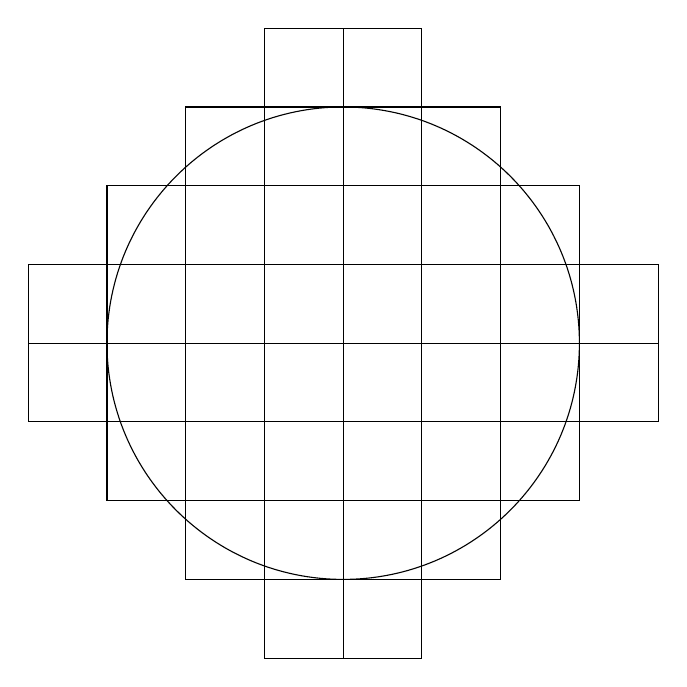
\begin{tikzpicture}[x=1cm]
			\foreach \y in {-5,...,5}{
				\foreach \x in {-5,...,5}{
					\pgfmathparse{abs(\y-0.5) + abs(\x-0.5)}
					\ifnum 5 > \pgfmathresult
					\draw (\x,\y) rectangle (\x,\y) rectangle (1+\x,1+\y);
					\fi
				}
			}
			\draw (1,1) circle (3);
		\end{tikzpicture}
	}
	\subfigure{
		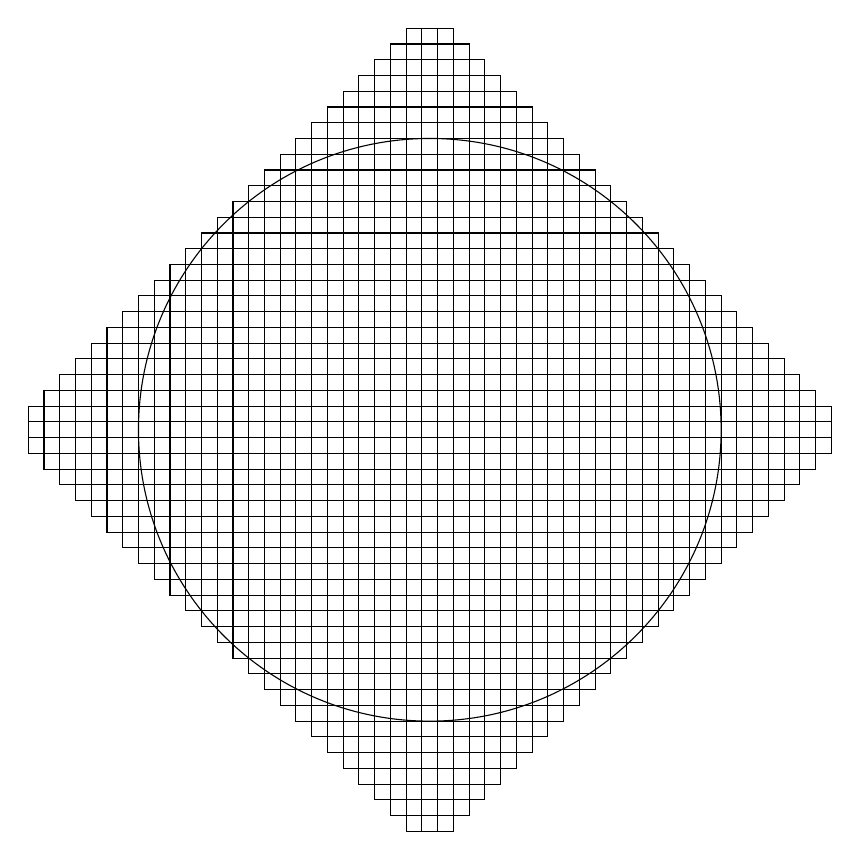
\begin{tikzpicture}[x=1cm]
			\foreach \y in {-25,...,25}{
				\foreach \x in {-25,...,25}{
					\pgfmathparse{abs(\y)-1 + abs(\x)-1}
					\ifnum 25 > \pgfmathresult
					\draw (\x /5, \y /5) rectangle ++(0.2,0.2);
					\fi
				}
			}
			\draw (0.1,0.1) circle (3.7);
		\end{tikzpicture}
	}
\end{figure}
Assume that all tilings are equally likely. The first thing one might notice when plotting tilings is that the most common tilings have a quirky behaviour: They freese the borders and stay random at a circle in the center.
\begin{figure}[h]
	\centering
	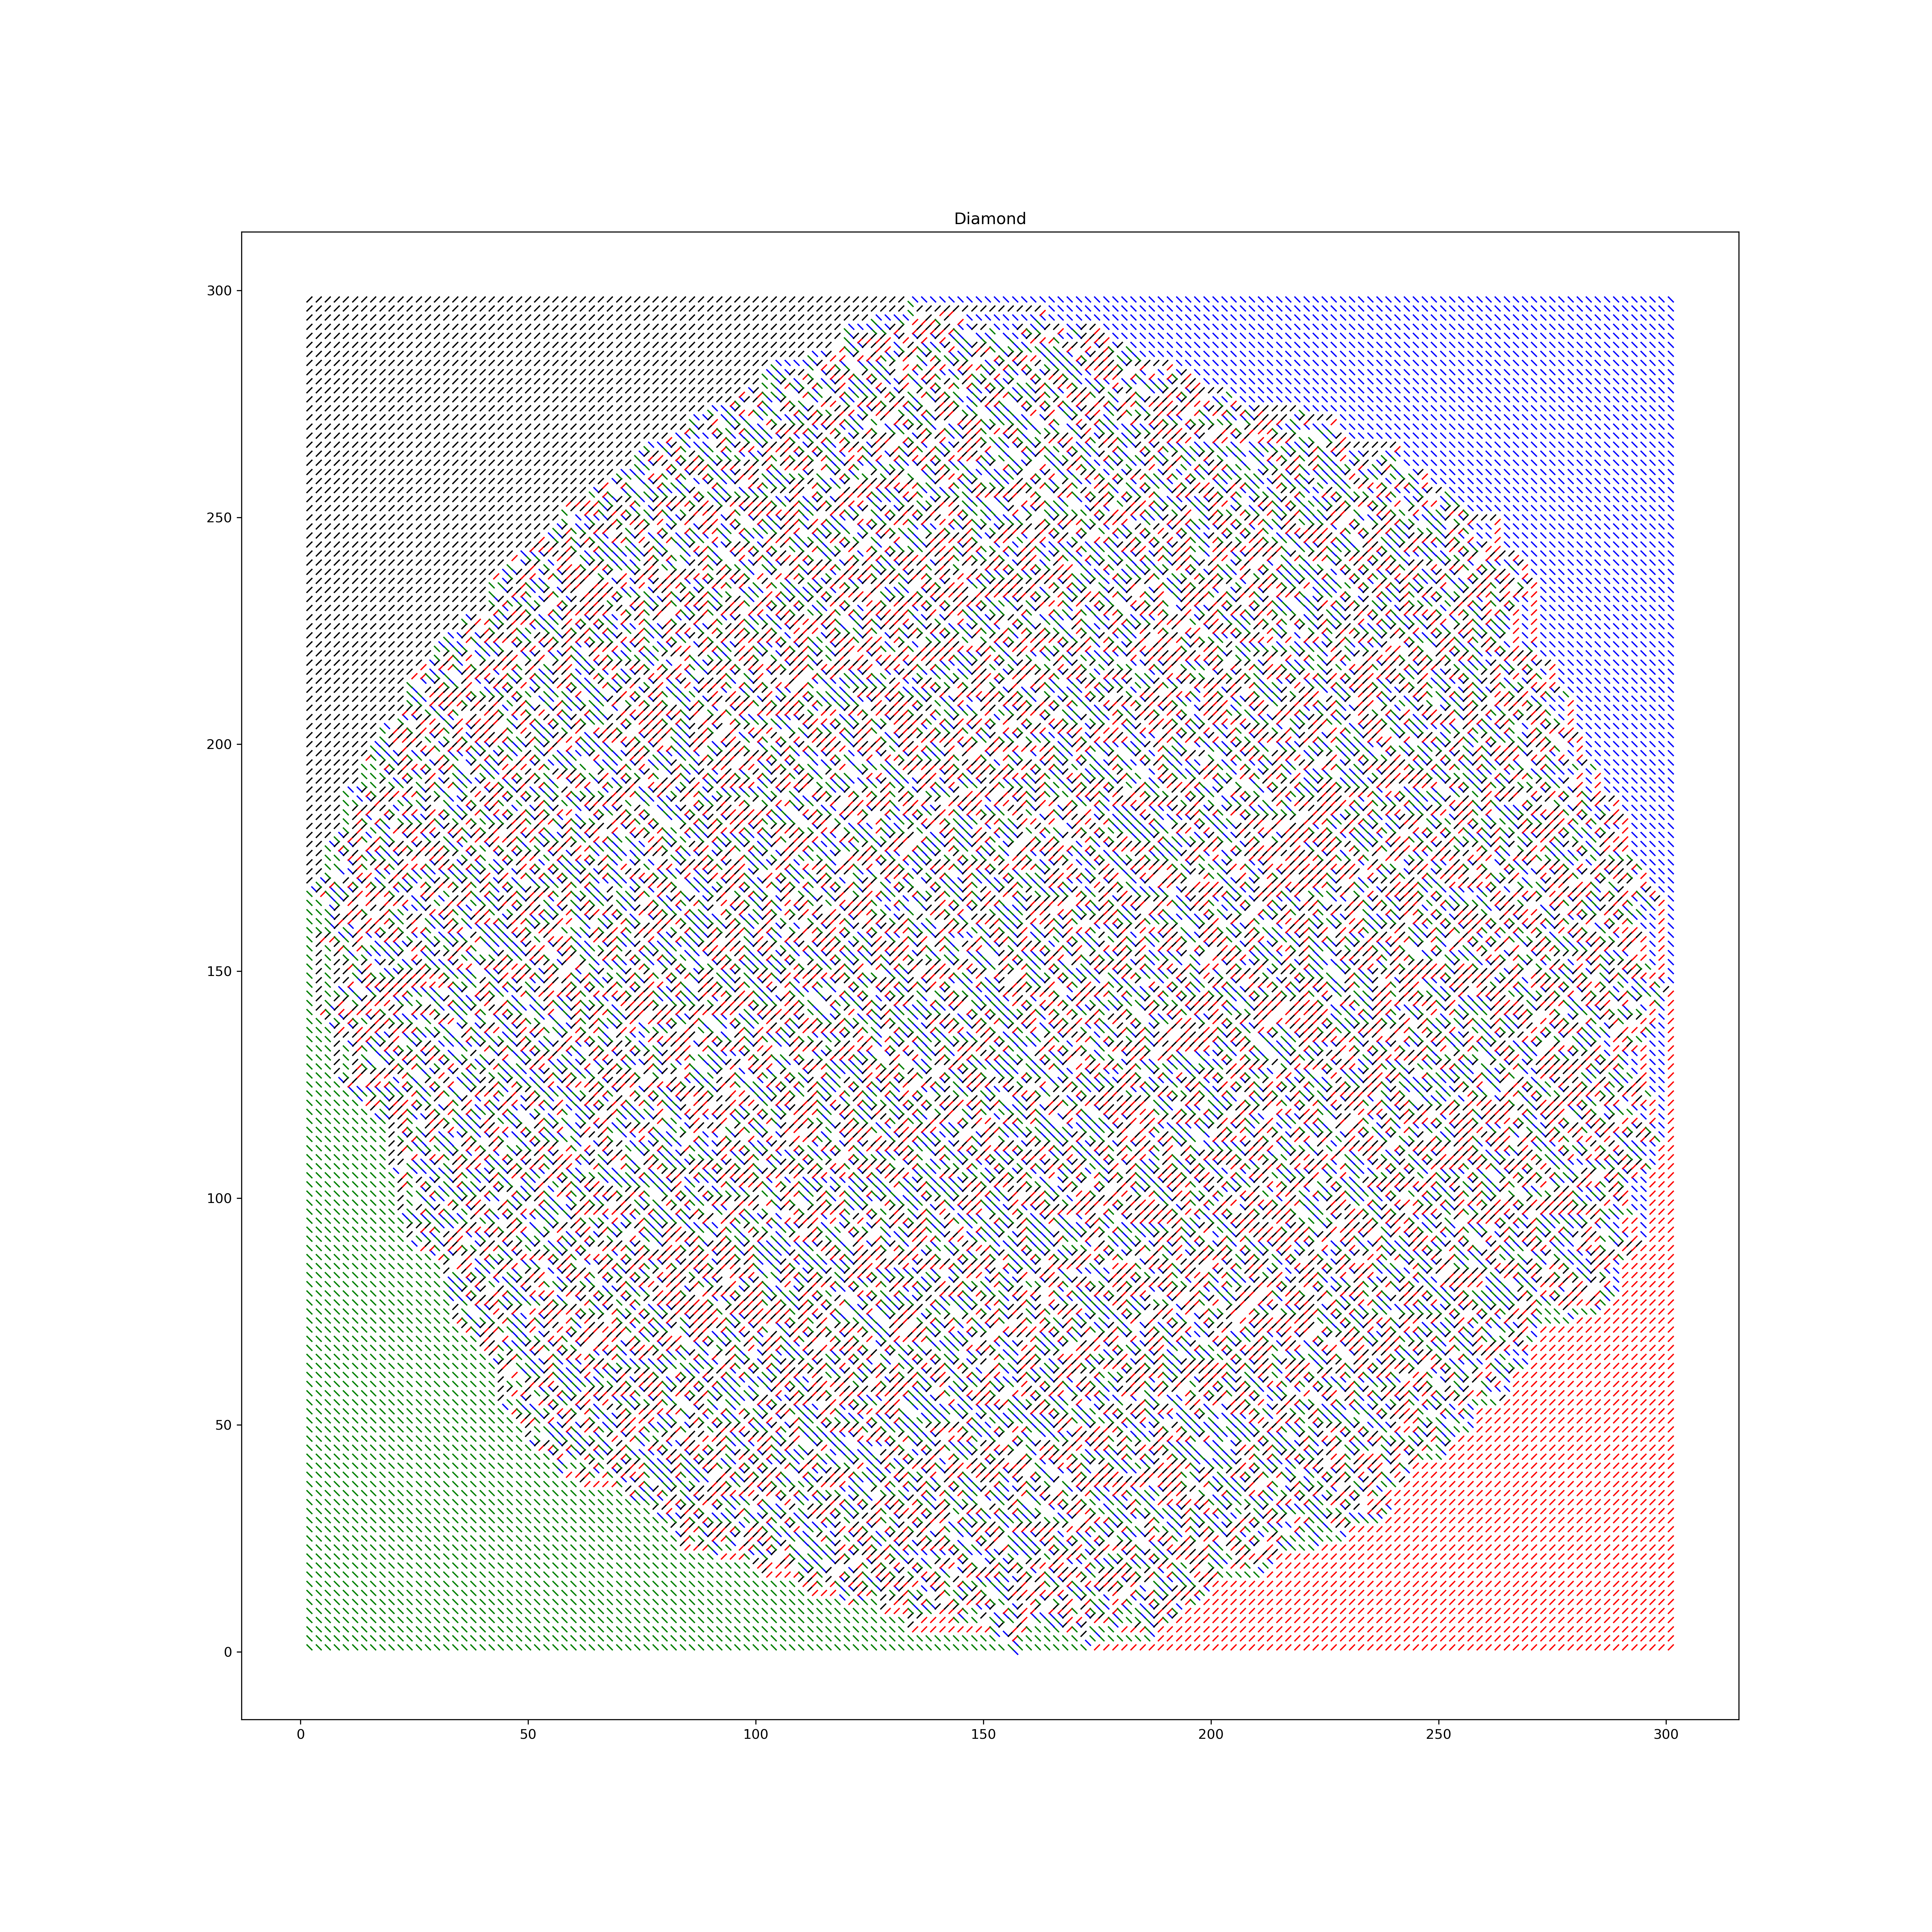
\includegraphics[width=0.7\linewidth]{./Assets/AstecDiamond.png}
\end{figure}
This is formally expressed in \cite{10.1214/10-AOP628}, 
\begin{thm}
	(The Article circle Theorem) FIz $\epsilon > 0$. FOr each $n$, consider a uniformly random domino tiling of the Astec Diamond of size $n$ scaçed by the factor $1/n$ in each axis to fit into the limiting diamond
	\begin{equation}
		AD_\infty \deff \{ |x| + |y| \leq 1\}
	\end{equation}
	and let $P_n^0 \subset n^{-1}AD_n$ be the image of the polar regions of the random tiling under this scaling transformation. Then as $n \rightarrow \infty$ the event that
	\begin{equation}
			\{(x, y) \in AD_\infty : x^2 + y^2 > \frac{1}{2} + \epsilon\} \bigcap (n^{-1} AD_n ) \subset P^0_n \subset \{(x, y) \in AD_\infty : x^2 + y^2 > \frac{1}{2} - \epsilon\}
	\end{equation}
	holds with probability that tends to $1$.
\end{thm}
The interesting result is in how much the border of the random region - or temperate, as some authors call it - deviates from the Artic Circle as $N$ grows large. For $-1 < \alpha < 1$ and $\alpha \neq 0$, let
\begin{equation}
		(x_\alpha^+, y_\alpha^+) = \left( 	\frac{\alpha + \sqrt{1-\alpha^2}}{2} , \frac{\alpha + \sqrt{1+\alpha^2}}{2}\right) \quad \text{and}, \quad (x_\alpha^-, y_\alpha^-) = \left( 	\frac{\alpha - \sqrt{1-\alpha^2}}{2} , \frac{\alpha + \sqrt{1+\alpha^2}}{2}\right) 
\end{equation}
denote the two points of intersection of the line $u + v = \alpha$ with $C_0 = \{u^2 + v^2 = \frac{1}{2}\}$. Then for fixed $\alpha$, Johansson showed that the fluctuations of the boundary of the temperate zone along the line $u + v = \alpha$ about the points $(x_\alpha^+ , y_\alpha^+ )$ and $(x_\alpha^- , y_\alpha^-)$ were described by the Tracy-Widom distribution $F_2$.

\section{Ulam's Problem}

This section is based on the Notes of the MasterClass given in Angers, France (2024) by Mattia Cafasso and Sofia Tarricone.

Let us consider the symmetric group $S_N$ of the permutations of the finite set $\{1, 2, \cdots, N\}$.
\begin{definition}
	Let $\pi \in S_n$ be a permutation. Given $k$ integers
	\begin{equation}
		1 \leq i_1 \leq i_2 \leq \cdots \leq i_k \leq N
	\end{equation}
	we say that $\pi(i_1), \cdots, \pi(i_k)$ is an incresing subsequence of $\pi$ of lenght $k$ if $\pi$ preserves the order of th eintegers $i_j$, $j = 1, \cdots, k$, i.e.
	\begin{equation}
		\pi(i_1) < \pi(i_2) < \cdots < \pi(i_k).
	\end{equation}
\end{definition}
We denote $l_N(\pi)$ the maximal lenght of all th eincreasing subsequences of $\pi$.

\begin{ex}
	Let $\pi = 54172386$. Then (by direct inpection), $l_N(\pi) = 4$. The maximal leght sequences are $(1, 2, 3, 6)$ and $(1, 2, 3, 8)$.
\end{ex}

Some history on the problem can be ennunciated as

\begin{enumerate}
	\item Stanislaw Ulam, in an article published in 1961, discussed the idea of using Monte Carlo approaches to study the asymptotic behavior of $\E[l_N]$, when $N \rightarrow \infty$. Based on his simulations, Ulam conjectured that it exists a constant $c$ such that $$\lim_{N \rightarrow \infty} \frac{\E[l_N]}{\sqrt{N}} = c.$$ The term Ulam's problem, originally, referred to the proof of this conjecture and the identifcation of the constant $c$. 
	\item Hammersley, in 1972, introduced a Poissonized version of this problem and proved that the constant $c$ exists. 
	\item In 1977, Logan and Shepp and, independently, Vershik and Kherov showed that $c = 2$. 
	\item Odlyzko and Rains, in the $90$'s, performed analytical simulations indicating that 
	\[
		\lim_{N \rightarrow \infty} \frac{\Var[l_N]}{N^{\frac{1}{3}}} = c_0 \equiv 0,819\cdots
	\]
	and also that
	\[
	\lim_{N \rightarrow \infty} \frac{\E[l_N] - 2\sqrt{N}}{N^{\frac{1}{6}}} = c_1 \equiv -1.748\cdots
	\]
\end{enumerate}

Finally, Ulam's problem was solved by Baik, Deift and Johansson in $1999$, who studied the convergence in distribution of the rescaled variable 
\begin{equation}
	\chi_N \deff \frac{l_N - 2\sqrt{N}}{N^{\frac{1}{6}}}
\end{equation}
given by
\begin{thm}
	(Baik-Deift-Johansson, $1999$). Let $\chi$ be a random variable with distribution function $F_{GUE}(x)$. Then $\chi_N$, defined as before, converges in distribution to $\chi$: 
	\begin{equation}
		\lim_{N \rightarrow \infty} \p\left\{ \frac{l_N - 2\sqrt{N}}{N^{\frac{1}{6}}} \leq x\right\} \rightarrow F_{(2)}(x)
	\end{equation}
	we have, moreover, convergence of moments
	\begin{equation}
			\lim_{N \rightarrow \infty} \E[\chi_N^m] = \E[\chi^m], \ \forall m \geq 1.
	\end{equation}
\end{thm}

To study, there is a nice representation of the permutated sequences that is worth exploring.

\subsection{Young's Diagram - and Tableaus}

Consider the following process. Start with a deck of $N$ well shuffled cards (with uniform measure) - numered $1, 2, \cdots, N$ for convenience. Now place the first card of the shuffled deck on the table. The second card will be placed on top of the first, if it is labelled with a smaller number, and on its side if it is labelled with a larger number. Now, if the third card is smaller than the two cards, it is again placed on top of both cards. If it is inbetween it is placed on the side of the second card. If it is bigger than both, it is placed on the side of the first card. The fourth card follows the same process. This gives rise to what we call a \textit{Young's Diagram}.

\begin{definition}
	A partition $\lambda = (\lambda_1, \cdots, \lambda_r)$ of $N$ is a set of positive integers such that $\lambda_1 \geq \lambda_2 \geq  \cdots \geq \lambda_r$ and $|\lambda| \deff \sum_i \lambda_i = N$. We call $|\lambda|$ the size of the partition, and $r$ its length. We will sometimes write $\lambda \vdash N$ to indicate that $\lambda$ has size $N$. 
\end{definition}

A convenient graphic representation of integer partitions is given by Young diagrams, which are constructing stacking r rows of boxes, each of length $\lambda_i$, in decreasing order. For instance, the partition $(5, 5, 3, 3, 2, 1, 1) \vdash 20$ corresponds to the Young diagram below: 
\begin{figure}[h!]
	\centering
	\ydiagram{5,5,3,3,2,1,1}
	\caption{Young Diagram}
\end{figure}
The set of Young diagrams of size $N$ will be denoted $YN$, and the set of all Young diagrams $Y$. From now on, we will implicitly identify a partition and the corresponding Young diagram. 

\begin{definition}
	A Young tableau of size $N$ is a Young diagram $(\lambda_1, \cdots, \lambda_r) \vdash N$ together with a bijection between its boxes and the integers $\{1, \cdots , N\}$. A standard Young tableau is a Young tableau whose integers increase along the lines and the columns. We will denote with $SYT_N$ the set of standard Young tableau of size $N$. The Young diagram of a given Young tableau $P$, denoted $\sh(P)$, is called the shape of the tableau. 
\end{definition}

\begin{ex}
	The two Young tableaux below are of shape $(5, 5, 4, 2, 2, 1) \vdash 19$, the first one is standard and the second one is not. 
	\begin{figure}[h!]
		\centering
		\subfigure{
			\begin{ytableau}
				1 & 3 & 4 & 8 & 10 \\
				2 & 5 & 9 & 13 & 14 \\
				6 & 11 & 12 & 16 \\
				7 & 15 \\
				17 & 18 \\
				19 \\
			\end{ytableau}
		}
		\subfigure{
			\begin{ytableau}
				5 & 3 & 4 & 8 & 10 \\
				2 & 1 & 12 & 13 & 14 \\
				6 & 11 & 9 & 16 \\
				15 & 7 \\
				17 & 18 \\
				19 \\
			\end{ytableau}
		}
		\caption{Young Tableau}
	\end{figure}
\end{ex}
\begin{thm}
If we define 
\begin{equation}
	F_\lambda \deff \{P \in SYT_N \ : \ \sh(P) = \lambda \}
\end{equation}	
we have the following (amazing) identity
\begin{equation}
	\sum_{\lambda \vdash N} F_\lambda^2 = N!
\end{equation}
derived using the so called Robinson-Schensted correspondence beetwen Young's Tableau and permutations,
\begin{equation}
	RS \ : \ S_N\rightarrow \{(P, Q) \in SYT_N \times SYT_N \ : \ \sh(P) = \sh(Q) \}
\end{equation}
\end{thm}

The interesting part we want to discuss is when we actually change the convention a little for the YOung Tableau. Namely, geometrically, we will rotate the diagram fourty five degrees and centralize the bottom corner to be at the origin of a Real line. Now, we associate the $YT$ with the following set of numbers: If we have the $YT - (\lambda_1, \cdots, \lambda_n)$, then teh set is given by 
\begin{equation}
	S(YT) = \left\{ \frac{\lambda_1 - 1}{2}, \frac{\lambda_2 - 3}{2}, \frac{\lambda_3 - 5}{2}, \cdots \right\}
\end{equation}
as depicted in the figure.
\begin{figure}[h!]
	\centering
	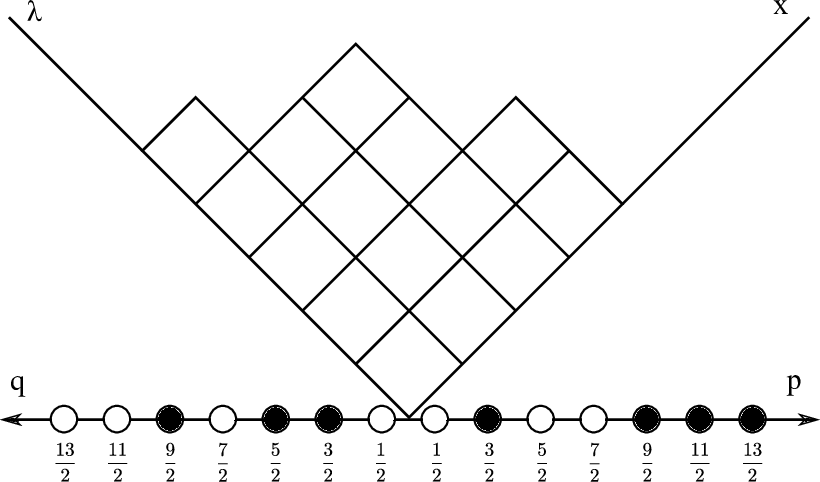
\includegraphics{./Assets/YoungTableauRotated.png}
\end{figure}
When we take the size of the $YT$ to be going to infinity we have a limiting shape represented below - this shape is well described.
%\begin{figure}[h!]
%	\centering
%	\subfigure{
%		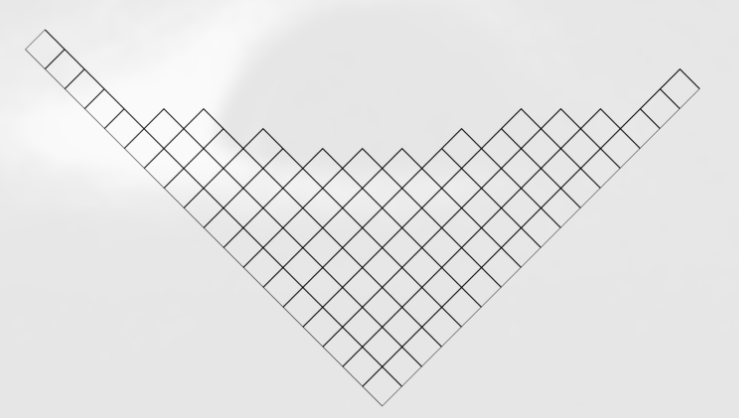
\includegraphics[width=0.45\linewidth]{./Assets/YTsmall.png}
%	}
%	\subfigure{
%		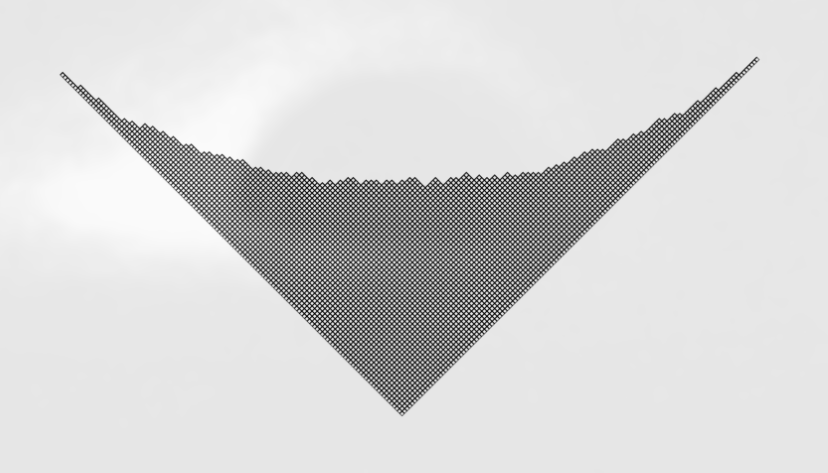
\includegraphics[width=0.45\linewidth]{./Assets/YTlarge.png}
%	}
%\end{figure}
More interesting, we also have a limit distribution of associated points $S(YT)$. This is excitely the same distribution of point we get for the eigenvalues of a matrix ensemble called Wigner Matrices.

\section{Matching Sequences}

This section is based on the work on \cite{majumdar2007randommatricesulamproblem}.

A very commom - and wildely important - method used in evolutionary biology, and man correlated areas, is the alignement of sequences. The goal of this method is to search for similarities in patters in different sequences. A classic, and commonly studied alignment problem is the so called 'longest common subsequence' (LCS). The setup is of two n- sequence and $m$- seuquence, composed of $n$ and $m$ letters, respectively, of the same $c$-alphabet (a set of $c$ letters).  This set could be, for example, the set of basis of the DNA.  Consider the sequences $\alpha, \beta$ given by
\begin{align*}
	\alpha \quad & : \qquad A \quad C \quad G \quad C \quad T \quad A \quad C \\
	\beta \quad & : \qquad C \quad T \quad G \quad A \quad C
\end{align*}
A subsequence of $\alpha$ is an ordered sublist of $\alpha$ (entries of which need not be consecutive in $\alpha$), e.g, $\{C, G, C, T\}$, but not $\{T, G, C\}$. A common subsequence of two sequences $\alpha$ and $\beta$ is a subsequence of both of them. For example, the subsequence $\{C, G, A, C\}$ is a common subsequence of both $\alpha$ and $\beta$. The aim of the LCS problem is to find the longest of such common subsequences between two fixed sequences $\alpha$ and $\beta$. 

A particularly important application of the LCS problem is to quantify the closeness between two DNA sequences. In evolutionary biology, the genes responsible for building specifci proteins evolve with time and by fniding the LCS of the same gene in different species, one can learn what has been conserved in time. Also, when a new DNA molecule is sequenced in vitro, it is important to know whether it is really new or it already exists. This is achieved quantitatively by measuring the LCS of the new molecule with another existing already in the database. 

For a pair of fixed sequences of length $i$ and $j$ respectively, the length $L_{i,j}$ of their LCS is just a number. However, in the stochastic version of the LCS problem one compares two random sequences drawn from $c$-alphabets and hence the length $L_{i,j}$ is a random variable. A major challenge over the last three decades has been to determine the statistics of $L_{i,j}$. For equally long sequences $(i = j = n)$, it has been proved that $\langle L_{n,n} \rangle \approx \gamma c n$ for $n \gg 1$, where the averaging is performed over all realizations of the random sequences. The constant $\gamma_c$ is known as the Chvátal-Sankoff constant which, to date, remains undetermined though there exists several bounds, a conjecture due to Steele that $\gamma_c = 2 / (1 + \sqrt{n})$ and a recent proof that $\gamma_c \rightarrow 2 / \sqrt{c} $ as $c \rightarrow \infty$. Unfortunately, no exact results are available for the finite size corrections to the leading behavior of the average $\langle L_{n,n} \rangle$, for the variance, and also for the full probability distribution of $L{n,n}$. Thus, despite tremendous analytical and numerical efforts, exact solution of the random LCS problem has, so far, remained elusive. Therefore it is important to fnid other variants of this LCS problem that may be analytically tractable. 

Computationally, the easiest way to determine the length $L_{i,j}$ of the LCS of two arbitrary sequences of lengths $i$ and $j$ (in polynomial time $O(ij)$) is via using the recursive algorithm
\begin{equation}
	 L_{i,j} = \max[L_{i-1,j}, L_{i,j-1}, L_{i-1,j-1}+ \eta_{i,j}] 
\end{equation}
 subject to the initial conditions $L_{0,j} = L_{i,0} = L_{0,0} = 0$. The variable $\eta_{i,j}$ is either $1$ when the characters at the positions $i$ (in the sequence $\alpha$) and $j$ (in the sequence $\beta$) match each other, or $0$ if they do not. Note that the variables $\eta_{i,j}$’s are not independent of each other. These residual correlations between the $\eta_{i,j}$ variables make the LCS problem rather complicated. Note however that for two random sequences drawn from $c$ alphabets, these correlations between the $\eta_{i,j}$ variables vanish in the $c \rightarrow \infty$ limit. 

A natural question is how important are these correlations between the $\eta_{i,j}$ variables, e.g., do they affect the asymptotic statistics of $L_{i,j}$’s for large $i$ and $j$? Is the problem solvable if one ignores these correlations? These questions naturally lead to the Bernoulli matching (BM) model which is a simpler variant of the original LCS problem where one ignores the correlations between $\eta_{i,j}$’s for all $c$. The length LBM $i,j$ of the BM model satisfeis the same recursion relation as before, except that $\eta_{i,j}$’s are now independent and each drawn from the bimodal distribution: $\p(\eta) = (1/c) \delta_{\eta,1} + (1-1/c) \delta_{\eta,0}$. This approximation is expected to be exact only in the appropriately taken $c \rightarrow \infty$ limit. Nevertheless, for finite $c$, the results on the BM model can serve as a useful benchmark for the original LCS model to decide if indeed the correlations between $\eta_{i,j}$’s are important or not. Unfortunately, even in the absence of correlations, the exact aymptotic distribution of $LBM_{i,j}$ in the BM model has so far remained elusive, mainly due to the nonlinear nature of the recursion relation. 

The reference presents present an exact asymptotic formula for the distribution of the length $LBM_{n,n}$ in the BM model for all $c$. So far, only the leading asymptotic behavior of the average length in the BM model was known using the ‘cavity’ method of spin glass physics,
\begin{equation}
	 \langle L^{(BM)}_{n,n} \rangle \approx \gamma^{(BM)}_c n
\end{equation}
where $\gamma_c^{(BM)} = 2/(1+\sqrt{c})$, the same as the conjectured value of the Chvátal-Sankoff constant $\gamma_c$ for the original LCS model. However, other properties such as the variance or the distribution of $LBM_{n,n}$ remained untractable even in the BM model. We have shown, as illustrated below, that for large $n$,
\begin{equation}
LBM_{n,n} \rightarrow \gamma^{(BM)}_c n + f(c) n^{1/3} \chi	
\end{equation}
where $\chi$ is a random variable with a $n$-independent distribution, $\p(\chi \leq x) = F_2(x)$, which is precisely the Tracy-Widom distribution.

Thus, the Tracy-Widom distribution also describes the asymptotic distribution of the optimal matching length in the BM model, for all $c$. Given that the correlations in the original LCS model become negligible in the $c \rightarrow \infty$ limit, it is likely that the BM asymptotics would also hold for the original LCS model in the $c \rightarrow \infty$. An important open problem is to determine whether the Tracy-Widom distribution also appears in the LCS problem for finite $c$. The distribution obtained for all $c$ in the BM model can serve as a useful benchmark to which future simulations of the LCS problem can be compared. 

\section{Public Transportation - Humam made}

The city of Cuernavaca in Mexico (population about $500.000$) has an extensive bus system, but there is no municipal transit authority to control the city transport. In particular there is no timetable, which gives rise to Poisson-like phenomena, with bunching and long waits between buses. Typically, the buses are owned by drivers as individual entrepreneurs, and all too often a bus arrives at a stop just as another bus is loading up. The driver then has to move on to the next stop to find his fares. In order to remedy the situation the drivers in Cuernavaca came up with a novel solution: they introduced “recorders” at specific locations along the bus routes in the city. The recorders kept track of when buses passed their locations, and then sold this information to the next driver, who could then speed up or slow down in order to optimize the distance to the preceding bus. The upshot of this ingenious scheme is that the drivers do not lose out on fares and the citizens of Cuernavaca now have a reliable and regular bus service. In the late $1990$’s two Czech physicists with interest in transportation problems, M. Krbalek and P. Seba, heard about the buses in Cuernavaca and went down to Mexico to investigate. For about a month they studied the statistics of bus arrivals on Line $4$ close to the city center. In particular, they studied the bus spacing distribution, and also the bus number variance measuring the fluctuations of the total number of buses arriving at a fixed location during a time interval $T$.

Krbalek and Seba found that both the bus spacing distribution and the number
variance are well modeled by GUE. In order to provide a plausible explanation of the observations in, the authors in introduced a microscopic model for the bus linethat leads simply and directly to GUE.

The main features of the bus system in Cuernavaca are
\begin{enumerate}
	\item the stop-start nature of the motion of the buses,
	\item the “repulsion” of the buses due to the presence of recorders.
\end{enumerate}
To capture these features, the authors introduced a model for the buses consisting of $n$ (number of buses) independent, rate $1$ Poisson processes moving from the bus depot at time $t = 0$ to the final terminus at time $T$, and conditioned not to intersect for $0 \leq t \leq T$. The authors then showed that at any observation point $x$ along the route of length $N > n$, the probability distribution for the (rescaled) arrival times of the buses, $y_j = \frac{2tj}{T} - 1 \in [-1, 1]$ for $i < j < n$ is given by
\begin{equation}
	c \prod_{j=1}^{n} w_J(y_j) \prod_{1 \leq i < j \leq n} (y_i - y_j)^2 \dd y_1 \cdots \dd y_n
\end{equation}
where
\begin{equation}
	w_J(y) = (1 + y)^{x-1} (1 - y)^{N-x-n+1}, \quad -1 < y < 1
\end{equation}
This formula is precisely the eigenvalue distribution for the so-called Jacobi Unitary Ensemble . In the appropriate scaling limit, GUE then emerges by universality. The authors also compute the distributions of the positions $x_1, \cdots , x_n$ of the buses at any time $t \in (0, T)$. Again the statistics of the $x_j$’s are described by a Unitary Ensemble, but now $w_J$ is the same, but replaced by the weight for the Krawtchouk polynomials: by universality, GUE again emerges in the appropriate scaling limit.

In an intriguing recent paper, Abul-Magd [Abu] noted that drivers have a tendency “to park their cars near to each other and at the same time keep a distance sufficient for manoeuvring.” He then analyzed data measuring the gaps between parked cars on four streets in central London and showed quite remarkably that the gap size distribution was well represented by the spacing distribution of GUE. It is an interesting challenge to develop a microscopic model for the parking problem, analogous to the model for the bus problem.

\section{Riemann zeta function - An anedote}
Here we consider the work of H. Montgomery in the early $1970$’s on the zeros of the Riemann zeta function $\zeta(s)$. Assuming the Riemann hypothesis, Montgomery rescaled the imaginary parts $\gamma_1 \leq \gamma_2 \leq \cdots$ of the (nontrivial) zeros $\{ 1/2 + \ii \gamma_j\}$ of $\zeta(s)$,
\[
\gamma_j \rightarrow \tilde{\gamma}_j = \frac{\gamma_j \log{\gamma_j}}{2\pi}
\]
to have mean spacing $1$ as $T \rightarrow \infty$, i.e.
\[
\lim_{T \rightarrow \infty} \frac{\#\{j \geq 1 : \tilde{\gamma}_j \leq T\}}{T} = 1
\]
For any $a < b$, he then computed the two-point correlation function for the $\tilde{\gamma}_j$’s
\[
\#\{\text{ordered pairs} (j_1, j_2), j_1 \neq j_2 : 1 \leq j_1, j_2 \leq N, \tilde{\gamma}_1 - \tilde{\gamma}_2 \in (a, b)\}
\]
and showed, modulo certain technical restrictions, that
\[
R(a, b) \equiv \lim_{N \rightarrow \infty}\frac{1}{N} \#\{\text{ordered pairs} (j_1, j_2), j_1 \neq j_2 : 1 \leq j_1, j_2 \leq N, \tilde{\gamma}_1 - \tilde{\gamma}_2 \in (a, b)\}
\]
exists and is given by a certain explicit formula. Soon after completing his work on the scaling limit (40) of the two-point correlation function for the zeros of zeta, Montgomery was visiting the Institute for Advanced Study in Princeton and it was suggested that he show his result to Dyson. What happened is a celebrated, and oft repeated, story in the lore of the Institute: before Montgomery could describe his hard won result to Dyson, Dyson took out
a pen, wrote down a formula, and asked Montgomery “And did you get this?”
\[
R(a, b) = \int_{a}^{b} 1 - \left( \frac{\sin(\pi r)}{\pi r}\right)^2 \dd r
\]
Montgomery was stunned: this was exactly the formula he had obtained. Dyson explained: “If the zeros of the zeta function behaved like the eigenvalues of a random GUE matrix, then would be exactly the formula for the two-point correlation function!”

\section{But what is the Tracy-Widow}

First of all, the expected value of this distribution is actually negative. Second of all, it is highly asymmetric, with the tail on the left decaying as $\exp(-|x|^3 /12)$ and the tail on the right decaying as $\exp(-4x^{3/2}/3)$. It is also worth noting that the range of validity of this distribution goes to zero as $N \rightarrow \infty$, since we scaled by $N^{1/6}$. We thus need a different tool to examine the part of the distribution where $|\lambda_{max} - \sqrt{2N} | > \Boh(N^{-1/6})$. These tails for large but finite $N$ have a dependence that goes as $e^{-N^2}$ on the left side and $e^{-N}$ on the right.

Recently, Majumdar and Schehr have shown that $N$ is large but finite, the Tracy-Widom distribution describes the crossover function between stable and unstable regimes of a random
dynamical system, and furthermore that there is a third order phase transition between these regimes, which also occurs in the Coulomb gas, two-dimensional QCD, and several other systems of physical interest. The universality of the Tracy-Widom distribution could be related to the universality of phase transitions — events such as water freezing into ice, graphite becoming diamond and ordinary metals transforming into strange superconductors.

\begin{figure}[h!]
	\centering
	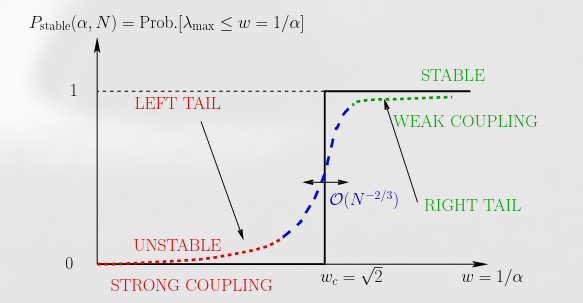
\includegraphics[width=0.5\linewidth]{./Assets/RegimeTW.png}
\end{figure}

In the thermodynamic equations describing water, the curve that represents the water’s energy as a function of temperature has a kink at 100 degrees Celsius, the point at which the liquid becomes steam. The water’s energy slowly increases up to this point, suddenly jumps to a new level and then slowly increases again along a different curve, in the form of steam. Crucially, where the energy curve has a kink, the “first derivative” of the curve has a peak.

Similarly, the physicists realized, the energy curves of certain strongly correlated systems have a kink at $\sqrt{2N}$. The associated peak for these systems is the Tracy-Widom distribution, which appears in the third derivative of the energy curve — that is, the rate of change of the rate of change of the energy’s rate of change. This makes the Tracy-Widom distribution a “third-order” phase transition.
